\documentclass[a4paper,10pt, dvipsnames]{report}

\usepackage{bookmark}
\usepackage[utf8]{inputenc}
\usepackage[T1]{fontenc}
\usepackage[scaled]{helvet}
\usepackage{amsmath} % Für Mathe
\usepackage{minted} % Für Codeblöcke
\usepackage[most]{tcolorbox} % Für farbige Boxen
\tcbuselibrary{minted} % tcolorbox Bibliothek für minted
\usepackage{hyperref} % Für Hyperlinks
\usepackage{geometry} % Für Seitenränder
\usepackage[ngerman]{babel} % Für deutsche Sprache
\usepackage{enumitem} % Für individuelle Listen
\usepackage{xcolor} % Für Farben
\usepackage{parskip}
\usepackage{titlesec}
\usepackage{hyperref}
\usepackage{longtable}
\usepackage[boxed]{algorithm2e}

\usepackage[
    type={CC},
    modifier={by-nc-sa},
    version={4.0},
]{doclicense}


\usepackage{fontawesome5}

\makeatletter
\newcommand{\github}[1]{%
   \href{#1}{\faGithubSquare}%
}
\makeatother


\titleformat{\chapter}[block]
  {\normalfont\huge\bfseries}
  {} % Kein Label wie "Kapitel"
  {0pt}
  {}

\hypersetup{
    colorlinks=true, % Färbt die Links statt einer Box um den Link
    linkcolor=black,  % Farbe der internen Links
    citecolor=green, % Farbe der Zitate
    filecolor=magenta, % Farbe für Dateilinks
    urlcolor=cyan   % Farbe der externen Links
}

\renewcommand\familydefault{\sfdefault}
\geometry{a4paper, left=20mm, right=20mm, top=20mm, bottom=20mm}

% tcolorbox Definition für Java-Codeblöcke
\newtcblisting{javacodebox}[1][]{
    listing engine=minted,
    colframe=black!70,
    listing only,
    minted style=colorful,
    minted language=java,
    minted options={tabsize=2,#1},
    left=1mm,
    boxsep=2mm,
    sharp corners,
    enhanced
}

\newcommand{\javaInLine}[1]{\mintinline[style=colorful]{java}{#1}}



% tcolorbox Definition für Text-Codeblöcke
\newtcblisting{textcodebox}[1][]{
    listing engine=minted,
    colback=ProcessBlue!20,
    colframe=black!70,
    listing only,
    minted style=colorful,
    minted language=text,
    minted options={tabsize=2,#1},
    left=1mm,
    boxsep=2mm,
    sharp corners,
    enhanced
}



\title{Programmierung 1}
\author{Lukas Batschelet (16-499-733)}
\date{HS 2023}

\begin{document}

\begin{titlepage}
    \begin{center}
        {\huge Programmierung 1}\\[0.5cm]
        {\large PD Dr. Kaspar Riesen}\\[0.3cm]
        {\LARGE Zusammenfassung \& Musterlösungen der Serien}\\[0.5cm]
        {\large HS 2023}\\[2cm]
        {\large Lukas Batschelet}\\[0.3cm]
        {\normalfont 16-499-733}\\[0.3cm]
    \end{center}
    \vfill % Fügt vertikalen Abstand ein, um den Text nach unten zu verschieben
    \noindent \github{https://github.com/lbatschelet/23HS_P1} Sämtliches Material ist auch auf GitHub abgelegt: \href{https://github.com/lbatschelet/23HS_P1}{https://github.com/lbatschelet/23HS\_P1}
    \doclicenseThis
\end{titlepage}

\tableofcontents

\chapter{Eigene Zusammenfasung}

\section{Grundlagen}

\subsection{Grundkonzepte der Java-Programmierung}

\begin{itemize}
    \item \textbf{Programmieren}: Problemlösung mit Software.
    \item \textbf{Programmiersprache}: Definiert mit Wörtern und Regeln Programmieranweisungen.
    \item \textbf{Java}: Weit verbreitet, vielseitig, plattformunabhängig, objektorientiert.
    \item \textbf{Klassen}: Grundbausteine von Java-Programmen; enthalten Methoden und Variablen.
    \item \textbf{main Methode}: Startpunkt jedes Java-Programms.
    \item \textbf{Kommentare}: Erläutern den Code (\javaInLine{//}, \javaInLine{/* */}, \javaInLine{/** */}).
\end{itemize}



\subsection{Notationskonventionen}

\begin{itemize}
    \item \textbf{Variablennamen}: Beginnen mit Kleinbuchstaben, CamelCase für zusammengesetzte Namen. Beispiel: \javaInLine{meinAlter}.
    \item \textbf{Konstanten}: Großbuchstaben und Unterstriche. Beispiel: \javaInLine{MAX_WERT}.
    \item \textbf{Methodennamen}: Beginnen mit Kleinbuchstaben, CamelCase für zusammengesetzte Namen, oft Verben. Beispiel: \javaInLine{berechneAlter()}.
    \item \textbf{Klassennamen}: Beginnen mit Großbuchstaben, CamelCase für zusammengesetzte Namen. Beispiel: \javaInLine{Person}.
\end{itemize}



\subsection{Variablendeklaration und -zuweisung}

\begin{itemize}
    \item \textit{Variable} := Speicherort für einen Wert oder ein Objekt.
    \item Variablen müssen mit \textit{Datentyp} und \textit{Bezeichner} deklariert werden.
    \item Mit dem \textit{Zuweisungsoperator} werden deklarierten Variablen Werte zugewiesen: \javaInLine{int i = 17;}.
    \item \textbf{Deklaration}: Definiert Typ und Namen der Variable, z.B. \javaInLine{int seiten;}.
    \item \textbf{Zuweisung}: Weist der Variablen einen Wert zu, z.B. \javaInLine{seiten = 256;}.
    \item \textbf{Kombinierte Deklaration und Zuweisung}: \javaInLine{int seiten = 256;}.
    \item \textbf{Mehrere Variablen}: Gleichzeitige Deklaration, z.B. \javaInLine{int figures = 46, tables; tables = 17;}.
\end{itemize}

\begin{itemize}
	\item Lesen verändert Variablen niemals: \javaInLine{MAX\_POINTS * 5}
	\item \textit{Zuweisungsoperatoren} und das \textit{Inkrement/Dekrement} machen das Leben einfacher:
\end{itemize}

\begin{javacodebox}
points = points * 2;
points *= 2;

points = points + 1;
points++;
\end{javacodebox}



\subsection{Primitive Datentypen}

\begin{itemize}
    \item \javaInLine{byte}: 8-Bit Ganzzahl, Bereich -128 bis 127.
    \item \javaInLine{short}: 16-Bit Ganzzahl, Bereich -32,768 bis 32,767.
    \item \javaInLine{int}: 32-Bit Ganzzahl, Bereich -2\textsuperscript{31} bis 2\textsuperscript{31}-1.
    \item \javaInLine{long}: 64-Bit Ganzzahl, Bereich -2\textsuperscript{63} bis 2\textsuperscript{63}-1.
    \item \javaInLine{float}: 32-Bit IEEE 754 Fließkommazahl.
    \item \javaInLine{double}: 64-Bit IEEE 754 Fließkommazahl.
    \item \javaInLine{boolean}: Wahrheitswert, \javaInLine{true} oder \javaInLine{false}.
    \item \javaInLine{char}: 16-Bit Unicode-Zeichen.
\end{itemize}



\subsection{Casting in Java}

\begin{itemize}
    \item \textbf{Implizites Casting}: Automatische Konvertierung von kleineren zu größeren Datentypen, z.B. \javaInLine{int} zu \javaInLine{double}.
    \item \textbf{Explizites Casting}: Man. Konv. von gross zu klein, z.B. \javaInLine{double num = 12.34; int count = (int) num;}.
\end{itemize}



\subsection{Aliase und Abhängigkeiten}

\begin{itemize}
    \item \textbf{Primitive Datentypen}: Kopien von Variablen sind unabhängig.
\end{itemize}

\begin{javacodebox}
    int num1 = 17;
    int num2 = num1;
    num2 = 99;
    System.out.println(num1); // 17
    System.out.println(num2); // 99
\end{javacodebox}


\begin{itemize}
    \item \textbf{Objektvariablen}: Kopien von Variablen sind abhängig (Aliase).
\end{itemize}

\begin{javacodebox}
    Integer num1 = new Integer(17);
    Integer num2 = num1;
    num2.setValue(99);
    System.out.println(num1); // 99
    System.out.println(num2); // 99
\end{javacodebox}

\subsection{Arithmetische Operatoren und Reihenfolge}


\begin{figure}
    \centering
    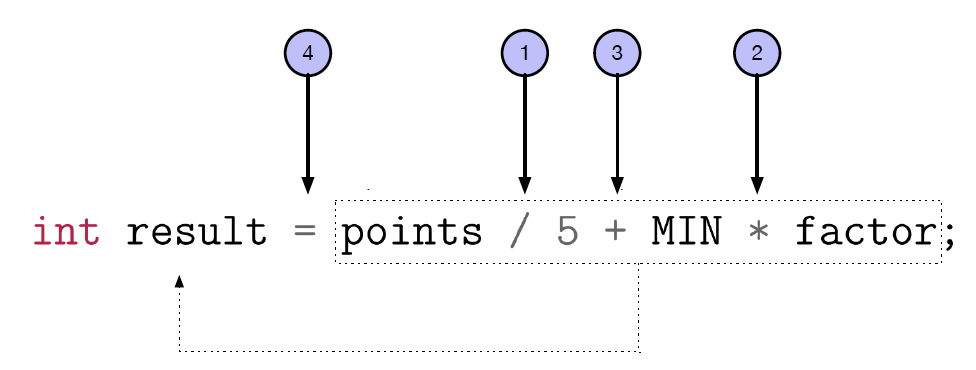
\includegraphics[width=0.5\linewidth]{resources/Operatorenreihenfolge.png}
    \caption{Reihenfolge der Auswertung: Der Zuweisungsoperator = hat die niedrigste Priorität.}
    \label{fig:Operatorenreihenfolge}
\end{figure}


\subsection{Division}

\begin{itemize}
    \item \textbf{Ganzzahldivision} (\javaInLine{int}):
    \begin{itemize}
        \item Das Ergebnis ist eine Ganzzahl, Bruchteile werden abgeschnitten.
        \item Beispiel: \javaInLine{int ergebnis = 5 / 2;} ergibt \javaInLine{2}.
    \end{itemize}

    \item \textbf{Fließkommadivision} (\javaInLine{double}):
    \begin{itemize}
        \item Das Ergebnis enthält Nachkommastellen.
        \item Beispiel: \javaInLine{double ergebnis = 5.0 / 2.0;} ergibt \javaInLine{2.5}.
    \end{itemize}

    \item \textbf{Casting bei Division}:
    \begin{itemize}
        \item Bei Casten einer Ganzzahldivision zu \javaInLine{double} bleibt der Bruchteil abgeschnitten.
        \item Beispiel: \javaInLine{double ergebnis = (double)(5 / 2);} ergibt \javaInLine{2.0}.
    \end{itemize}
\end{itemize}




\section{Java-Klassen}

\subsection{Aufbau einer Java-Klasse}

\begin{itemize}
    \item \textbf{Klassendefinition}: Beginnt mit dem Schlüsselwort \javaInLine{class}, gefolgt vom Klassennamen.
    \item \textbf{Attribute}: Variablen innerhalb einer Klasse, repräsentieren den Zustand.
    \item \textbf{Methoden}: Funktionen innerhalb einer Klasse, definieren Verhalten.
    \item \textbf{Konstruktor}: Spezielle Methode zum Erstellen von Objekten.
\end{itemize}

\begin{javacodebox}
    public class Auto {
        // Attribute
        private String marke;
        private int baujahr;
    
        // Konstruktor
        public Auto(String marke, int baujahr) {
            this.marke = marke;
            this.baujahr = baujahr;
        }
    
        // Methode
        public void anzeige() {
            System.out.println(marke + ", Baujahr: " + baujahr);
        }
    }
\end{javacodebox}

\begin{figure}
    \centering
    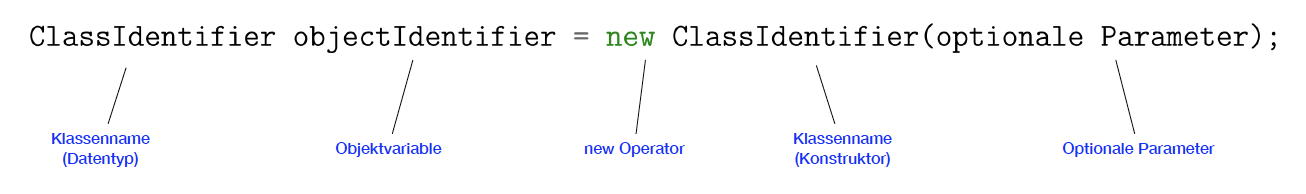
\includegraphics[width=0.75\linewidth]{resources/ObjektDeklarierungUndInstanziierung.png}
    \caption{Deklaration und Instanziierung eines Objektes.}
    \label{fig:deklaration-und-instanziierung}
\end{figure}



\subsection{Methodenkopf}

\begin{itemize}
    \item Methodenkopf: (1) Sichtbarkeit (2) Datentyp der Rückgabe oder void (3) Bezeichner (4) Formale Parameter in Klammern
    \item \textbf{Sichtbarkeitssmodifizierer}: Bestimmt die Sichtbarkeit (z.B. \javaInLine{public}, \javaInLine{private}).
    \item \textbf{Rückgabetyp}: Datentyp des Rückgabewerts der Methode.
    \item \textbf{Methodenname}: Eindeutiger Bezeichner der Methode.
    \item \textbf{Formale Parameterliste}: Variablen zur übergabe von Werten an die Methode.
    \item Variablen sollten \javaInLine{private} deklariert werden.
    \item Methoden können \javaInLine{private} oder \javaInLine{public} deklariert werden (je nach Zweck)
\end{itemize}



\begin{javacodebox}
public class Integer {

    private int value;

    public Integer(int value) {
    this.value = value;
    }
    public String toString() {
    return this.value + "";
    }
    public void setValue(int value) {
    this.value = value;
    }
}
\end{javacodebox}



\subsection{Konstruktoren}

\begin{itemize}
    \item \textbf{Definition}: Spezielle Methode zum Erstellen und Initialisieren eines Objekts.
    \item \textbf{Konstruktortypen}: Standardkonstruktor (ohne Parameter) und parametrisierte Konstruktoren.
\end{itemize}

\begin{javacodebox}
public class Auto {
    private String marke;
    private int baujahr;

    // Standardkonstruktor
    public Auto() {
    }

    // Parametrisierter Konstruktor
    public Auto(String marke, int baujahr) {
        this.marke = marke;
        this.baujahr = baujahr;
    }
}
\end{javacodebox}



\subsection{Parameter und variadische Methoden}

\begin{itemize}
    \item \textbf{Parameter}: Variablen, die beim Aufruf einer Methode Werte übergeben.
    \item \textbf{Variadische Parameter (Varargs)}: Erlauben eine variable Anzahl von Argumenten.
\end{itemize}

\begin{javacodebox}
public class Rechner {
    // Variadische Methode
    public int summe(int... zahlen) {
        int summe = 0;
        for (int zahl : zahlen) {
            summe += zahl;
        }
        return summe;
    }
}
\end{javacodebox}


\subsection{Generische Klassen}

\begin{itemize}
    \item Wir können Klassen generisch machen:
\end{itemize}

\begin{javacodebox}
public class Rocket<T> {

    private T cargo;

    public Rocket(T cargo) {
        this.cargo = cargo;
    }
    public void set(T cargo) {
        this.cargo = cargo;
    }
    public T get() {
        return this.cargo;
    }
}
\end{javacodebox}


\begin{itemize}
	\item Um eine generische Klasse zu instanziieren, müssen wir sie zusammen mit einem \textit{Typargument} instanziieren:
\end{itemize}

\begin{javacodebox}
    Rocket<Integer> intRocket = new Rocket<Integer>();
    Rocket<String> stringRocket = new Rocket<String>();
\end{javacodebox} 

\begin{itemize}
	\item Die Typvariable \javaInLine{T} wird nun überall mit dem Typargument ersetzt.
\end{itemize}



\subsection{\javaInLine{enum}}

\begin{itemize}
    \item Ein \javaInLine{enum} zählt \textit{alle} zulässigen Werte eines Typs auf
\end{itemize}

\begin{javacodebox}
    public enum Category {
        Mathematik, Geographie
    }
\end{javacodebox}

\begin{javacodebox}
    public enum Category {
        Mathematik(1), Geographie(2);
        private int id;
        private Category(int id) {
            this.id = id;
        }
        public int getId() {
            return this.id;
        }
    }
\end{javacodebox}

\begin{itemize}
    \item Jedes \javaInLine{enum} besitzt Methoden (wie z.B. \javaInLine{getId()})
    \item Jede \javaInLine{enum}-Klasse besitzt statische Methoden (wie z.B. \javaInLine{values()})
\end{itemize}

\begin{javacodebox}
    Category[] categories = Category.values();
    for (Category category : categories) {
        System.out.println(category);
    }
\end{javacodebox}


\subsection{Statische Variablen und Methoden}

\begin{itemize}
    \item Statische Variablen werden von allen Instanzen geteilt (es existiert also nur eine Kopie der Variablen für alle Objekte)
\end{itemize}

\begin{javacodebox}
    public class Person {
        public static int globalCount = 0;
        private int id;
        public Person() {
            this.id = Person.globalCount++;
        }
    }
\end{javacodebox}

\begin{itemize}
    \item Statische Methoden werden direkt aufgerufen, ohne vorher ein Objekt zu instanziieren
\end{itemize}

\begin{javacodebox}
    public class Math {
        public static int max(int a, int b) {
            return (a > b) ? a : b;
        }
    }
\end{javacodebox}

\begin{javacodebox}
    int max = Math.max(3, 7);
\end{javacodebox}



\subsection{Klassen des java-API}

\subsubsection{Wrapper-Klassen und Methoden}

\small

\begin{longtable}{|p{0.3\linewidth}|p{0.3\linewidth}|p{0.15\linewidth}|p{0.15\linewidth}|}
\hline
\textbf{Methode} & \textbf{Beschreibung} & \textbf{Bsp. Eingabe} & \textbf{Bsp. Rückgabe} \\
\hline
\endhead

% Integer Methoden
\multicolumn{4}{|l|}{\textbf{Integer}} \\
\hline
\javaInLine{parseInt(String s)} & Konvertiert String zu int & \javaInLine{"123"} & \javaInLine{123} \\
\javaInLine{valueOf(int i)} & Gibt Integer-Objekt für int-Wert & \javaInLine{123} & \javaInLine{Integer 123} \\
\javaInLine{compare(int x, int y)} & Vergleicht zwei int-Werte & \javaInLine{compare(3, 7)} & \javaInLine{-1} \\
\javaInLine{MIN_VALUE} & Gibt den kleinsten int-Wert & - & \javaInLine{-2147483648} \\
\javaInLine{MAX_VALUE} & Gibt den größten int-Wert & - & \javaInLine{2147483647} \\
\hline

% Double Methoden
\multicolumn{4}{|l|}{\textbf{Double}} \\
\hline
\javaInLine{parseDouble(String s)} & Konvertiert String zu double & \javaInLine{"123.45"} & \javaInLine{123.45} \\
\javaInLine{valueOf(double d)} & Gibt Double-Objekt für double-Wert & \javaInLine{123.45} & \javaInLine{Double 123.45} \\
\javaInLine{compare(double d1, double d2)} & Vergleicht zwei double-Werte & \javaInLine{compare(3.5, 7.5)} & \javaInLine{-1} \\
\javaInLine{POSITIVE_INFINITY} & Gibt den positiven unendlichen double-Wert & - & \javaInLine{Infinity} \\
\javaInLine{NEGATIVE_INFINITY} & Gibt den negativen unendlichen double-Wert & - & \javaInLine{-Infinity} \\
\hline

% Boolean Methoden
\multicolumn{4}{|l|}{\textbf{Boolean}} \\
\hline
\javaInLine{parseBoolean(String s)} & Konvertiert String zu boolean & \javaInLine{"true"} & \javaInLine{true} \\
\javaInLine{valueOf(boolean b)} & Gibt Boolean-Objekt für boolean-Wert & \javaInLine{true} & \javaInLine{Boolean true} \\
\hline

% Character Methoden
\multicolumn{4}{|l|}{\textbf{Character}} \\
\hline
\javaInLine{isLetter(char c)} & Prüft, ob Zeichen ein Buchstabe ist & \javaInLine{'a'} & \javaInLine{true} \\
\javaInLine{isDigit(char c)} & Prüft, ob Zeichen eine Ziffer ist & \javaInLine{'1'} & \javaInLine{true} \\
\javaInLine{toUpperCase(char c)} & Wandelt Zeichen in Großbuchstaben & \javaInLine{'a'} & \javaInLine{'A'} \\
\javaInLine{toLowerCase(char c)} & Wandelt Zeichen in Kleinbuchstaben & \javaInLine{'A'} & \javaInLine{'a'} \\
\hline

\end{longtable}

\normalsize


\subsubsection{weitere Klassen}

\small

\begin{longtable}{|p{0.3\linewidth}|p{0.3\linewidth}|p{0.15\linewidth}|p{0.15\linewidth}|}
\hline
\textbf{Klasse \& Methode} & \textbf{Beschreibung} & \textbf{Bsp. Eingabe} & \textbf{Bsp. Rückgabe} \\
\hline
\endhead

% String Methoden
\javaInLine{String.length()} & Gibt die Länge des Strings zurück & \javaInLine{"Hello"} & \javaInLine{5} \\
\javaInLine{String.charAt(int index)} & Gibt Zeichen an Index zurück & \javaInLine{"Hello", 1} & \javaInLine{'e'} \\
\javaInLine{String.substring(int a, int b)} & Gibt Teilstring zurück & \javaInLine{"Hello", 1, 3} & \javaInLine{"el"} \\
\javaInLine{String.indexOf(String str)} & Gibt Index des Teilstrings oder -1 & \javaInLine{"Hello", "ll"} & \javaInLine{2} \\
\javaInLine{String.toLowerCase()} & Konvertiert String zu Kleinbuchstaben & \javaInLine{"Hello"} & \javaInLine{"hello"} \\
\javaInLine{String.toUpperCase()} & Konvertiert String zu Großbuchstaben & \javaInLine{"hello"} & \javaInLine{"HELLO"} \\
\javaInLine{String.contains(CharSequence s)} & Prüft, ob String Teilstring enthält & \javaInLine{"Hello", "ll"} & \javaInLine{true} \\
\javaInLine{String.equals(Object anObject)} & Vergleicht zwei Strings & \javaInLine{"Hello", "hello"} & \javaInLine{false} \\
\hline

% Math Methoden
\javaInLine{Math.sqrt(double a)} & Quadratwurzel von a & \texttt{4} & \texttt{2.0} \\
\javaInLine{Math.pow(double a, double b)} & a hoch b & \texttt{2, 3} & \texttt{8.0} \\
\javaInLine{Math.abs(int a)} & Absolutwert von a & \texttt{-5} & \texttt{5} \\
\javaInLine{Math.random()} & Zufällige Zahl zwischen 0.0 und 1.0 & - & \texttt{0.45} \\
\hline

% Random Methoden
\javaInLine{Random.nextInt()} & Zufällige Ganzzahl & - & \texttt{42} \\
\javaInLine{Random.nextInt(int bound)} & Zufällige Ganzzahl bis bound (exkl.) & \texttt{10} & \texttt{5} \\
\javaInLine{Random.nextBoolean()} & Zufälliger Wahrheitswert & - & \texttt{true} \\
\javaInLine{Random.nextDouble()} & Zufällige Fließkommazahl & - & \texttt{0.62} \\
\hline

% System Methoden
\javaInLine{System.currentTimeMillis()} & Aktuelle Zeit in Millisekunden seit 1. Januar 1970 & - & \texttt{1609459200000} \\
\hline

% Scanner Methoden
\javaInLine{Scanner(System.in)} & Scanner für Eingaben & - & - \\
\javaInLine{Scanner.next()} & Liest das nächste Token & - & \texttt{"Hello"} \\
\javaInLine{Scanner.nextLine()} & Liest die nächste Zeile & - & \texttt{"Hello World"} \\
\javaInLine{Scanner.nextInt()} & Liest die nächste Ganzzahl & - & \texttt{42} \\
\hline

% DecimalFormat Methoden
\javaInLine{DecimalFormat(String pattern)} & Konstruktor mit Muster & \texttt{"\#0.00"} & - \\
\javaInLine{format(double number)} & Formatieren einer Zahl & \texttt{1234.5678} & \texttt{"1234.57"} \\
\hline
\end{longtable}

\begin{itemize}
    \item \textbf{\#} - Stellt eine Ziffer dar; Null wird nicht dargestellt, wenn sie nicht notwendig ist.
    \item \textbf{0} - Stellt eine Ziffer dar; führt zu Nullen, wenn keine Ziffer vorhanden ist.
    \item \textbf{.} - Dezimaltrennzeichen.
    \item \textbf{,} - Gruppierungstrennzeichen.
    \item \textbf{\%} - Multipliziert die Zahl mit 100 und zeigt sie als Prozentsatz an.
    \item \textbf{E0} - Trennt die Mantisse und Exponenten in wissenschaftlicher Notation.
    \item \textbf{;} - Trennt Formate; das erste für positive Zahlen und das zweite für negative Zahlen.
\end{itemize}

\normalsize

\subsection{\javaInLine{ArrayList<T>}}

\begin{itemize}
	\item Die Klasse \javaInLine{ArrayList<T>} erlaubt es, generische Sammlungen von Objekten des Typs \javaInLine{T} anzulegen.
\end{itemize}


\begin{itemize}
	\item Objekte dieser Klasse werden bei der Instanziierung parametrisiert:
\end{itemize}

\begin{javacodebox}
ArrayList<String> names = new ArrayList<String>();
ArrayList<PlayerCard> cards = new ArrayList<PlayerCard>();
ArrayList<Integer> numbers = new ArrayList<Integer>();
\end{javacodebox}

\begin{itemize}
	\item Listen passen Ihre Grösse dynamisch an:
\end{itemize}

\begin{javacodebox}
names.add("Keanu");
names.add("Kevin");
System.out.println(names); // [Keanu, Kevin]
names.add("Karl");
System.out.println(names); // [Keanu, Kevin, Karl]
names.remove(1);
System.out.println(names); // [Keanu, Karl]
\end{javacodebox}



\subsection{\javaInLine{PrintWriter}}

\begin{itemize}
	\item Die Klasse \javaInLine{PrintWriter} erlaubt Ausgaben in Dateien (wirft möglicherweise eine Exception)
\end{itemize}

\begin{javacodebox}
public static void main(String[] args) throws IOException {
    String fileName = "output.txt";
    PrintWriter outFile = new PrintWriter(fileName);
    outFile.print("Hallo Welt!");
    outFile.close();
}
\end{javacodebox}


\subsection{Abhängigkeit von sich selbst}

\begin{itemize}
    \item Eine Klasse kann von sich selbst abhängig sein
\end{itemize}

\begin{javacodebox}
public class Person {

    private String name;
    private ArrayList<Person> friends;

    public Person(String name) {
        this.name = name;
        this.friends = new ArrayList<Person>();
    }
    public void knows(Person other) {
        this.friends.add(other);
    }
    public String toString() {
        return this.name;
    }
    public ArrayList<Person> getFriends() {
        return this.friends;
    }
}
\end{javacodebox}

\begin{javacodebox}
Person p1 = new Person("Emilie");
Person p2 = new Person("Ava");
Person p3 = new Person("Maya");
p1.knows(p2);
p1.knows(p3);

System.out.println(p1.getFriends()); // [Ava, Maya]
\end{javacodebox}


\subsection{Aggregation}

\begin{itemize}
    \item Aggregation := Ein Objekt besteht z.T. aus anderen Objekten
\end{itemize}

\begin{javacodebox}
    public class Person {

    private String name;
    private Adress address;

    public Person(String name, Adress address) {
        this.name = name;
        this.address = address;
    }
}
\end{javacodebox}

\begin{javacodebox}
    public class Adress {

    private String street;
    private int zipCode;

    public Adress(String street, int zipCode) {
        this.street = street;
        this.zipCode = zipCode;
    }
}
\end{javacodebox}


\subsection{Getter und Setter}

\begin{itemize}
    \item \textbf{Getter}: Methode, die den Wert eines Attributs zurückgibt.
    \item \textbf{Setter}: Methode, die den Wert eines Attributs setzt.
\end{itemize}

\begin{javacodebox}
public class Auto {
    private String marke;

    // Getter
    public String getMarke() {
        return marke;
    }

    // Setter
    public void setMarke(String marke) {
        this.marke = marke;
    }
}
\end{javacodebox}



\section{Schleifen und Bedingungen}

\subsection{\javaInLine{if}-\javaInLine{else} Anweisung}

\begin{itemize}
    \item \textbf{Verwendung}: Zur Kontrolle des Programmflusses basierend auf Bedingungen.
    \item \textbf{Struktur}: Besteht aus einer Bedingung und einem Codeblock, der ausgeführt wird, wenn die Bedingung wahr (`true`) ist.
\end{itemize}

\begin{javacodebox}
if (bedingung) {
    // Code, der ausgeführt wird, wenn Bedingung wahr ist
} else {
    // Code, der ausgeführt wird, wenn Bedingung falsch ist
}
\end{javacodebox}



\subsection{\javaInLine{switch}-Anweisung}

\begin{itemize}
    \item \textbf{Verwendung}: Vereinfacht mehrfache `if-else`-Anweisungen, basierend auf dem Wert einer Variablen.
    \item \textbf{Struktur}: Besteht aus einem Ausdruck und mehreren `case`-Labels, die unterschiedliche Fälle repräsentieren.
\end{itemize}

\begin{javacodebox}
switch (variable) {
    case wert1:
        // Code für wert1
        break;
    case wert2:
        // Code für wert2
        break;
    default:
        // Code, wenn kein anderer Fall zutrifft
}
\end{javacodebox}



\subsection{Conditional Operator}

\begin{itemize}
    \item \textbf{Verwendung}: Kürzere Form für einfache `if-else`-Anweisungen.
    \item \textbf{Struktur}: Drei Teile - eine Bedingung, ein Ergebnis für `true` und ein Ergebnis für `false`.
\end{itemize}

\begin{javacodebox}
    int ergebnis = (bedingung) ? wertWennTrue : wertWennFalse;
\end{javacodebox}


\subsection{\javaInLine{do}-\javaInLine{while}-Schleife}

\begin{itemize}
    \item \textbf{Verwendung}: Schleife, die den Codeblock mindestens einmal ausführt und danach prüft, ob die Bedingung wahr ist.
    \item \textbf{Struktur}: Die Bedingung wird am Ende jeder Schleifeniteration überprüft.
\end{itemize}

\begin{javacodebox}
    do {
        // Code, der mindestens einmal ausgeführt wird
    } while (bedingung);
\end{javacodebox}



\subsection{\javaInLine{for}-Schleife}

\begin{itemize}
    \item \textbf{Verwendung}: Schleife mit definierter Anzahl von Iterationen.
    \item \textbf{Struktur}: Besteht aus Initialisierung, Bedingung und Inkrementierung.
    \item \textbf{For-Schleife}: Klassische Schleife mit definierter Anzahl von Iterationen.
    \item \textbf{For-Each-Schleife}: Vereinfachte Form zum Durchlaufen von Arrays oder Sammlungen.
    \item Der \textit{Schleifenkopf} der \javaInLine{for}-Schleife besteht aus drei Teilen:
    \begin{itemize}
        \item \textit{Initialisierung}: Wird am Anfang und genau einmal durchgeführt.
        \item \textit{Boolesche Bedingung}: Wird immer vor dem nächsten Eintritt in die Schleife überprüft.
        \item \textit{Inkrement}: Wird immer am Ende der Schleife durchgeführt.
    \end{itemize}
\end{itemize}

\begin{javacodebox}
    // Klassische For-Schleife
    for (int i = 0; i < 10; i++) {
        // Code, der 10 Mal ausgeführt wird
    }

    // For-Each-Schleife
    int[] zahlen = {1, 2, 3, 4, 5};
    for (int zahl : zahlen) {
        // Code, der für jede Zahl im ArrayList-Element ausgeführt wird
    }
\end{javacodebox}

\subsection{Vergleiche}

\begin{itemize}
    \item Vorsich bei \javaInLine{==} auf Dezimalzahlen
\end{itemize}

\begin{javacodebox}
    final double TOLERANCE = 0.00000001;
    if (Math.abs(num1 - num2) < TOLERANCE) {
        // ...
    }
\end{javacodebox}

\begin{itemize}
    \item Vergleich von Zeichen basiert auf Unicode (Ziffern < Grossbuchstaben < Kleinbuchstaben)
\end{itemize}

\begin{javacodebox}
    char c0 = '0', c1 = 'A', c2 = 'a';
    System.out.println(c0 < c1); // true
    System.out.println(c1 < c2); // true
\end{javacodebox}

\begin{itemize}
    \item Vorsicht bei \javaInLine{==} auf Objekten: Testet auf Aliase
    \item Verwenden/Schreiben der Methode \javaInLine{equals} und der Methode \javaInLine{compareTo}
\end{itemize}

\begin{javacodebox}
    public class Integer {
        private int value;
        public Integer(int value) {
            this.value = value;
        }
        public boolean equals(Integer other) {
            return this.value == other.value;
        }
        public int compareTo(Integer other) {
            return this.value - other.value;
        }
    }
\end{javacodebox}

\begin{javacodebox}
    Integer i1 = new Integer(2);
    Integer i2 = new Integer(17);
    Integer i3 = new Integer(2);
    System.out.println(i1.equals(i2)); // false
    System.out.println(i1.equals(i3)); // true

    System.out.println(i1.compareTo(i2)); // -15
    System.out.println(i1.compareTo(i3)); // 0
    System.out.println(i2.compareTo(i3)); // 15
\end{javacodebox}

\subsubsection{Wächterwerte}

\begin{itemize}
    \item Mit \textit{Wächterwerten} können wir ein Programm kontrollieren:
\end{itemize}

\begin{javacodebox}
    Scanner scan = new Scanner(System.in);
    int input = 1;
    while (input != 0) {
        System.out.print("Mit 0 Beenden Sie den Prozess. ");
        input = scan.nextInt();
    }
    System.out.println("--ENDE--");
\end{javacodebox}

\begin{itemize}
    \item \javaInLine{while}-Schleifen können auch zur Kontrolle von Eingaben verwendet werden:
\end{itemize}

\begin{javacodebox}
    Scanner scan = new Scanner(System.in);
    System.out.print("Alter eingeben: ");
    int age = scan.nextInt();
    while (age < 0) {
        System.out.println("Ungültiger Wert.");
        System.out.print("Alter eingeben: ");
        age = scan.nextInt();
    }
\end{javacodebox}

\subsection{\javaInLine{do}-Anweisung}

\begin{itemize}
    \item Die \javaInLine{do}-Anweisung ist ähnlich zur \javaInLine{while}-Anweisung, evaluiert aber die Boolesche Bedingung am Ende der Schleife.
\end{itemize}

\begin{javacodebox}
    System.out.print("Erreichte Punkte (0 bis 100): ");
    int points = scan.nextInt();
    while (points < 0 || points > 100) {
        System.out.print("Erreichte Punkte (0 bis 100): ");
        points = scan.nextInt();
    }
\end{javacodebox}

\begin{javacodebox}
    int points;
    do {
        System.out.print("Erreichte Punkte (0 bis 100): ");
        points = scan.nextInt();
    } while (points < 0 || points > 100);
\end{javacodebox}

\subsection{Vergleich von Daten}

\begin{itemize}
    \item \textbf{Primitive Datentypen}: Verwendung von Vergleichsoperatoren wie \javaInLine{==}, \javaInLine{!=}, \javaInLine{<}, \javaInLine{>}.
    \item \textbf{Objekte}: Implementierung der \javaInLine{compareTo()} Methode aus dem \javaInLine{Comparable} Interface.
\end{itemize}

\begin{javacodebox}
    // Vergleich von primitiven Datentypen
    int x = 5;
    int y = 10;
    boolean sindGleich = x == y; // false

    // Implementierung von compareTo
    public class Person implements Comparable<Person> {
        private int alter;

        @Override
        public int compareTo(Person anderePerson) {
            return Integer.compare(this.alter, anderePerson.alter);
        }
    }
\end{javacodebox}


\section{Arrays}

\begin{itemize}
	\item Arrays ermöglichen das Deklarieren einer einzigen Variablen eines Typs, die dann mehrere Werte dieses Typs speichern kann
	\item Arrays haben eine feste, unveränderliche Grösse (Konstante \javaInLine{length}), die bei der Instanziierung angegeben werden muss
\end{itemize}

\begin{javacodebox}
    int num1, num2, num3, num4, num5, num6;

    int[] nums = new int[6];

    int l = nums.length;
\end{javacodebox}

\begin{itemize}
	\item Auf einzelne Elemente eines Arrays greift man mit einem Index innerhalb eckiger Klammern zu
\end{itemize}

\begin{javacodebox}
    for (int i = 0; i < nums.length; i++) {
        System.out.println(nums[i]);
\end{javacodebox}


\subsection{Instanziierung}

\begin{itemize}
	\item Mit Initialisierungslisten können Arrays instanziiert und mit Werten gefüllt werden
\end{itemize}

\begin{javacodebox}
    int[] nums = {1, 2, 3, 4};
    String[] names = {"Goodbye", "Hello", "Hi", "Howdy"};
\end{javacodebox}


\begin{itemize}
	\item Auf Methoden der in einem Array gespeicherten Objekte kann man über Array-Referenzen zugreifen
\end{itemize}

\begin{javacodebox}
    for (int i = 0; i < names.length; i++)
        names[i] = names[i].toUpperCase();
\end{javacodebox}


\begin{itemize}
	\item Der Parameter der Methode \javaInLine{main} ist ein \javaInLine{String[]}. Dies sind Programmparameter, die beim Start des Programmes von "Aussen" mitgegeben werden können
\end{itemize}

\begin{javacodebox}
    public static void main(String[] args) {
        String language = args[0];
        String version = args[1];
        String author = args[2];
    }
\end{javacodebox}

\subsection{Variable Parameterlisten}

\begin{itemize}
    \item Methoden können mit variablen Parameterlisten umgehen
\end{itemize}

\begin{javacodebox}
    public static int min(int first, int ... others) {
        int min = first;
        for (int num : others)
            min = Math.min(min, num);
        return min;
    }
\end{javacodebox}

\begin{javacodebox}
    public class Greetings {
        private String primaryGreeting;
        private String[] greetings;
        public Greetings(String primaryGreeting, String ... otherGreetings) {
            this.primaryGreeting = primaryGreeting;
            this.greetings = otherGreetings;
        }
    }
\end{javacodebox}


\subsection{Mehrdimensionale Arrays}

\begin{itemize}
	\item Zweidimensionale Arrays sind Arrays aus Arrays
\end{itemize}

\begin{javacodebox}
    int[][] table = new int[100][5];
    String[][] names = {{"Anne", "Barbara", "Cathrine"}, {"Danny", "Emilie", "Fanny"}};
\end{javacodebox}

\begin{itemize}
	\item Für Referenzen auf Elemente in zweidimensionalen Arrays werden zwei Indizes benötigt
\end{itemize}


\begin{javacodebox}
    System.out.println(names[0][2]);
    for (int row = 0; row < names.length; row++)
        for (int col = 0; col < names[row].length; col++)
            names[row][col] = "Hannes";
\end{javacodebox}


\section{Schnittstellen und Vererbung}

\subsection{Schnittstellen}

\begin{itemize}
	\item Schnittstellen enthalten abstrakte Methoden und/oder Konstanten
\end{itemize}

\begin{javacodebox}
    public interface Eatable {
        void eat();
    }
\end{javacodebox}


\begin{itemize}
	\item Sie verleihen unterschiedlichen Dingen eine gemeinsame Sichtweise, ein gemeinsames Verhalten
\end{itemize}

\begin{javacodebox}
    public class BrusselsSprouts implements Eatable {
\end{javacodebox}

\begin{javacodebox}
    public class Potato implements Eatable {
\end{javacodebox}

\begin{javacodebox}
    public class Chocolate implements Eatable {
\end{javacodebox}


\begin{itemize}
	\item Polymorphes Verhalten via Schnittstellen
\end{itemize}

\begin{javacodebox}
    Eatable[] storage = new Eatable[3];
    storage[0] = new Chocolate();
    storage[1] = new BrusselsSprouts();
    storage[2] = new Potato();
    for (Eatable eatable : storage)
        eatable.eat();
\end{javacodebox}


\begin{itemize}
	\item Schnittstellen erlauben auch das Verbergen von Implementationsdetails und den Austausch von Klassen
\end{itemize}

\begin{minipage}{0.48\linewidth}
\begin{javacodebox}
public interface Bag {
    void add(Item item);
}
\end{javacodebox}

\begin{javacodebox}
public class BackPack implements Bag {
    private ArrayList<Item> items;

    public void add(Item item) {
        this.items.add(item);
    }
}
\end{javacodebox}

\begin{javacodebox}
Bag bag = new BackPack();
bag.add(new Item("Socken"));
bag.add(new Item("Hosen"));
bag.add(new Item("Shirt"));
\end{javacodebox}
\end{minipage}
\hfill % Fügt einen horizontalen Zwischenraum zwischen den minipages ein
\begin{minipage}{0.48\linewidth}
\begin{javacodebox}
public class SuitCase implements Bag {
    private int numberOfItems;
    private Item[] items;

    public SuitCase() {
        this.numberOfItems = 0;
        this.items = new Item[100];
    }
    public void add(Item item) {
        this.items[numberOfItems] = item;
        this.numberOfItems++;
    }
}
\end{javacodebox}

\begin{javacodebox}
Bag bag = new SuitCase();
bag.add(new Item("Socken"));
bag.add(new Item("Hosen"));
bag.add(new Item("Shirt"));
\end{javacodebox}
\end{minipage}



\subsection{Vererbung}

\begin{itemize}
	\item Vererbung ist eines der Kernkonzepte der objektorientierten Programmierung
	\item In Java ist nur Einfachvererbung erlaubt
	\item Vererbung ist eine Einbahnstrasse
	\item Geerbte Methoden/Variablen werden weitervererbt
	\item Abstrakte Klassen dienen als Platzhalter in Hierarchien
\end{itemize}

\begin{figure}
    \centering
    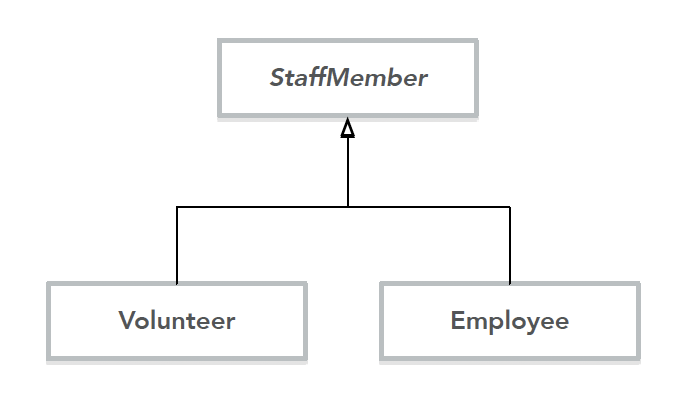
\includegraphics[width=0.5\linewidth]{resources/Vererbung.png}
\end{figure}


\begin{itemize}
	\item Im Konstruktor der Subklasse wird immer als erstes der Konstruktor der Superklasse aufgerufen
	\item Geerbte Methoden können überschrieben werden
	\item Eine konkrete Subklasse einer abstrakten Klasse muss alle abstrakten Methoden implementieren
	\item Mit der Referenz \javaInLine{super} kann auf die Superklasse zugegriffen werden
\end{itemize}

\scriptsize
\begin{minipage}{0.48\linewidth}
\begin{javacodebox}
public abstract class StaffMember {

    protected String name;

    public StaffMember(String name) {
        this.name = name;
    }
    public abstract double pay();

    public String toString() {
        return this.name;
    }
}
\end{javacodebox}

\begin{javacodebox}
public class Volunteer extends StaffMember {
    public Volunteer(String name) {
        super(name);
    }
    public double pay() {
        return 0;
    }
}
\end{javacodebox}
\end{minipage}
\hfill
\begin{minipage}{0.48\linewidth}
\begin{javacodebox}
public class Employee extends StaffMember {

    protected String socialSecurityNumber;
    protected double payRate;

    public Employee(String name,
            String socialSecurityNumber,
            double payRate) {
        super(name);
        this.socialSecurityNumber = socialSecurityNumber;
        this.payRate = payRate;
    }
    public double pay() {
        return this.payRate;
    }
    public String toString() {
        String s = super.toString();
        return s + " " + this.socialSecurityNumber;
    }
}
\end{javacodebox}
\end{minipage}
\normalsize

\subsection{Polymorphismus}


\begin{itemize}
	\item Die Variable \javaInLine{member} ist polymorph
\end{itemize}

\begin{javacodebox}
StaffMember member;
member = new Employee("Daniel", "123-456", 8300.00);
member = new Volunteer("Tobias");
\end{javacodebox}

\begin{itemize}
	\item Polymorphes Verhalten via Vererbung
\end{itemize}

\begin{javacodebox}
ArrayList<StaffMember> staff = new ArrayList<StaffMember>();
staff.add(new Employee("Daniel", "123-456", 8300.00));
staff.add(new Volunteer("Tobias"));
staff.add(new Volunteer("Susanne"));
staff.add(new Employee("Madeleine", "133-456", 15999.00));

for (StaffMember s : staff)
    s.pay(); // Polymorphes Verhalten
\end{javacodebox}


\section{Algorithmen und Methoden}

\subsection{Überladen von Methoden}

\begin{itemize}
    \item Methoden können überladen werden
    \item Methoden mit gleichem Namen, aber unterschiedlichen Parametern
    \item Signatur (:= Bezeichner + formale Parameter) muss eindeutig sein
    \item Rückgabetyp kann nicht überladen werden
\end{itemize}

\begin{javacodebox}
private void doThis(int val) {
}
private void doThis(int val1, int val2) {
}
private void doThis(double val) {
}
\end{javacodebox}

\subsection{Algorithmen}

\begin{itemize}
	\item Sortieren und Suchen sind zwei klassische Problemfelder der Informatik
	\item Es existieren zahlreiche Lösungen/Algorithmen für beide Problemfelder
\end{itemize}

\begin{algorithm}[H]
\DontPrintSemicolon
\caption{Selection-Sort(\textit{list})}

\For{$index = 0, \ldots, (\textit{list.length} - 2)$}{
    $min = index$\;
    \For{$scan = index + 1, \ldots, (\textit{list.length} - 1)$}{
        \If{$\textit{list}[scan] < \textit{list}[min]$}{
            $min = scan$\;
        }
    }
    \textit{Tauche list[index] mit list[min]}
}
\end{algorithm}

\subsection{Generische Typisierung}

\begin{itemize}
	\item Methoden können auch generisch programmiert werden:
\end{itemize}


\begin{javacodebox}
public static <T> void printArray(T[] array) {
    for (T element : array)
        System.out.println(element);
}
\end{javacodebox}


\begin{itemize}
	\item Die Typvariable \javaInLine{T} wird beim Aufruf der Methode definiert:
\end{itemize}

\begin{javacodebox}
Contact[] friends = new Contact[8];
…
Sorting.insertionSort(friends);
\end{javacodebox}

\subsection{Herrsche und Teile}

\begin{itemize}
	\item Jede Funktion, die ein Programm erfüllen soll, muss in einer Methode programmiert sein
	\item Komplexe Funktionalitäten sollten Sie in mehrere Teile zerlegen
	\begin{itemize}
        \item Verständlicher
        \item Wiederverwendbar
        \item leichter zu testen
        \item schneller erstellt
    \end{itemize}
\end{itemize}

\begin{javacodebox}
public static <T> void bubbleSort(Comparable<T>[] list) {
    for (int i = 0; i <= list.length - 2; i++)
        for (int j = list.length - 1; j >= i + 1; j--)
            if (list[j].compareTo((T) list[j - 1]) < 0)
                swap(list, j, j -1);
}

private static <T> void swap(Comparable<T>[] list, int j, int i) {
    Comparable<T> temp = list[j];
    list[j] = list[i];
    list[i] = temp;
}
\end{javacodebox}

\subsection{Rekursion}

\begin{itemize}
	\item Rekursion: Etwas ist durch sich selbst definiert
	\begin{itemize}
        \item \texttt{Liste := Zahl}
	    \item \texttt{Liste := Zahl, Liste}
    \end{itemize}
	\item Jede rekursive Definition benötigt einen nichtrekursiven Teil, den Basisfall, so dass die Rekursion enden kann
	\item Rekursive Methode: Die Methode ruft sich selber direkt oder indirekt auf
	\item Jeder rekursive Aufruf einer Methode definiert eigene lokale Variablen und eigene formale Parameter
\end{itemize}

\begin{minipage}{0.48\linewidth}
\begin{javacodebox}
public class Recursion {
    public static void main(String[] args) {
        System.out.println(f(5, 4));
    }

    public static double f(int n, int m) {
        if (m == 1)
            return n;
        else
            return f(n, m - 1) + n;
    }
}
\end{javacodebox}
\end{minipage}
\hfill
\begin{minipage}{0.48\linewidth}
    \begin{center}
        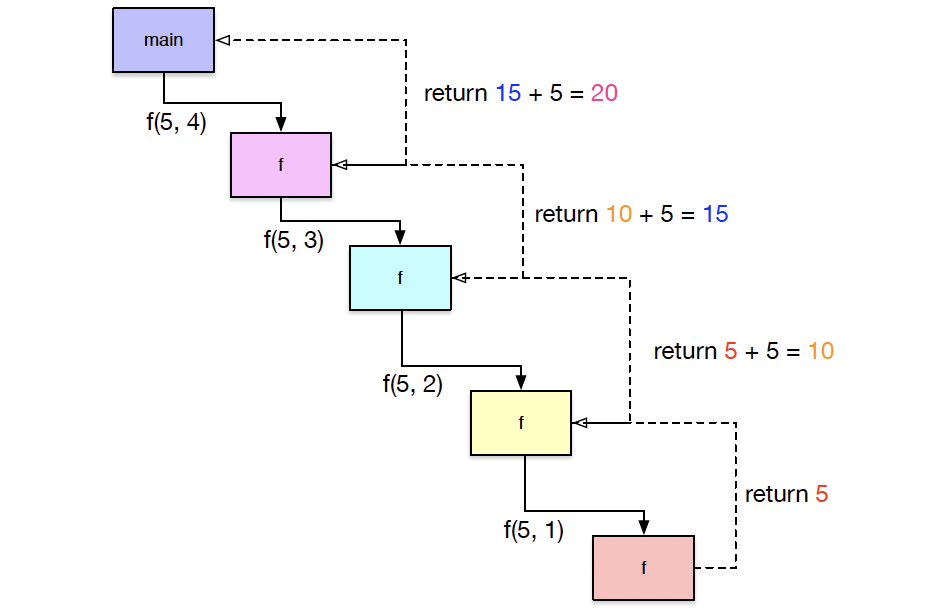
\includegraphics[width=1\linewidth]{resources/Rekursion.png}
    \end{center}
\end{minipage}


\begin{itemize}
	\item Mit Rekursion kann man einige Probleme elegant lösen
\end{itemize}

\begin{javacodebox}
public static <T> void quickSort(Comparable<T>[] list, int p, int r) {
    if (p < r) {
        int q = partition(list, p, r);
        quickSort(list, p, q - 1);
        quickSort(list, q + 1, r);
    }
}
\end{javacodebox}

\begin{itemize}
	\item Rekursive Algorithmen sind aber manchmal nicht so intuitiv wie iterative Algorithmen
\end{itemize}

\begin{javacodebox}
public static double f_1(int n, int m) {
    if (m == 1)
        return n;
    else
        return f_1(n, m - 1) + n;
}

public static double f_2(int n, int m) {
    return n * m;
}
\end{javacodebox}


\subsection{Testen}

\begin{itemize}
	\item Testen umfasst mindestens das Ausführen eines vollendeten Programms mit verschiedenen Eingaben
	\item Test Case := Eingaben und Benutzeraktionen, gekoppelt mit den erwarteten Ergebnissen
	\item Test Suite := Mehrere Test Cases
	\item Defekttest := Ziel ist es, Fehler zu finden
	\item Regressionstest: Ziel ist es, nach der Korrektur keine neuen Fehler einzubauen
	\item Black-Box Test: Beruht nur auf Eingaben und erwarteten Ausgaben
	\item White-Box Test: Konzentriert sich auf die interne Struktur des Codes
\end{itemize}


\section{Collection Framework}

\begin{itemize}
	\item Sammlung :=Behälter, um (meist gleichartige) Elemente zu organisieren.
	\item Idee einer Sammlung und die Implementierung sind zwei unterschiedliche Dinge
\end{itemize}

\begin{center}
    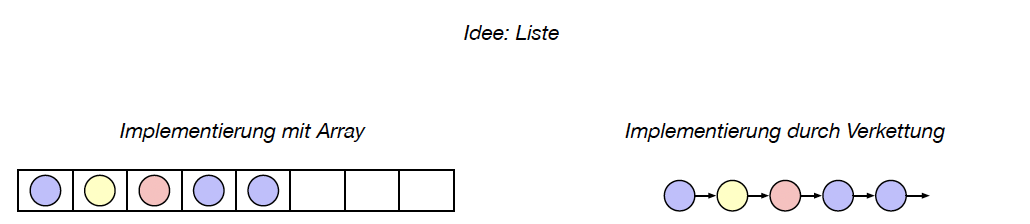
\includegraphics[width=0.75\linewidth]{resources/Idee_Implementierung.png}
\end{center}

\begin{itemize}
	\item Wichtige abstrakte Datentypen und deren Implementierungen im Java API:
	\begin{itemize}
        \item Listen (z.B. die Klasse \javaInLine{LinkedList})
        \begin{itemize}
            \item Verarbeitung über Index
        \end{itemize}
        \item Warteschlangen (z.B. die Schnittstelle \javaInLine{Queue})
        \begin{itemize}
            \item FIFO Verarbeitung
        \end{itemize}
        \item Stapel (z.B. die Klasse \javaInLine{Stack})
        \begin{itemize}
            \item LIFO Verarbeitung
        \end{itemize}
        \item Mengen (z.B. die Klasse \javaInLine{TreeSet})
        \begin{itemize}
            \item Keine Duplikate, keine Position
        \end{itemize}
        \item Assoziativspeicher (z.B. die Klasse \javaInLine{HashMap})
        \begin{itemize}
            \item Schlüssel-Wert Paare
        \end{itemize}
    \end{itemize}
\end{itemize}

\begin{center}
    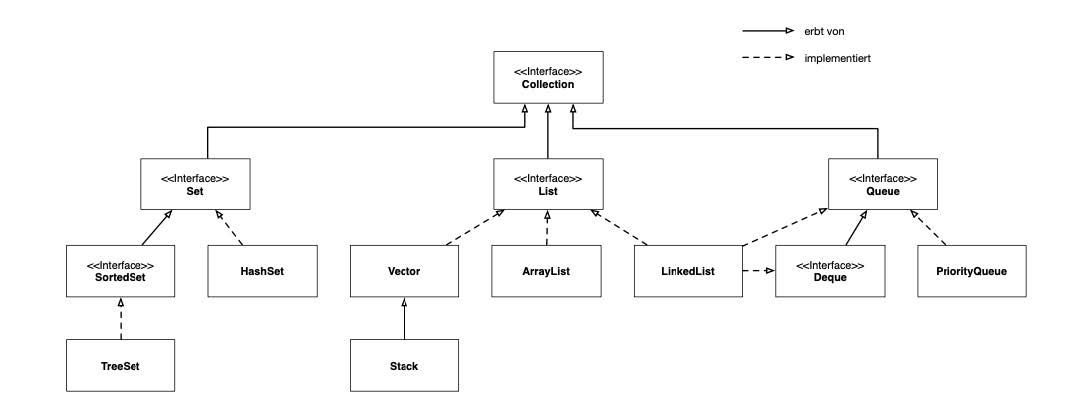
\includegraphics[width=\linewidth]{resources/CollectionFramework.jpg}
\end{center}

\begin{itemize}
	\item Das Collection Framework des Java APIs erlaubt die Trennung von abstrakten Datentypen (:= Schnittstellen) und Implementierungen
\end{itemize}

\begin{javacodebox}
List<Door> list = new ArrayList<Door>();

List<Door> list = new LinkedList<Door>();
\end{javacodebox}

\begin{itemize}
	\item Einige Methoden sind "weit oben" in der Hierarchie deklariert:
	\begin{itemize}
        \item \javaInLine{add(T t)} oder \javaInLine{size()}
    \end{itemize}
    \item Einige Methoden machen nur auf speziellen Datenstrukturen Sinn:
    \begin{itemize}
        \item \javaInLine{add(int index, T t)} oder \javaInLine{peekFirst()}
    \end{itemize}
\end{itemize}


\section{Laufzeitfehler}

\begin{itemize}
	\item Laufzeitfehler sind Objekte der Klasse \javaInLine{Exception}, die eine unübliche Situation repräsentieren
	\item Fehlermeldungen beinhalten den Namen der \javaInLine{Exception}, möglicherweise eine Nachricht, welche den Fehler umschreibt, sowie eine genaue Angabe, wo im Quellcode die \javaInLine{Exception} geworfen wurde
\end{itemize}

\begin{textcodebox}
exception in thread "main"
java.lang.ArithmeticException: / by zero at
ExceptionDemo.main(ExceptionDemo.java:11)
\end{textcodebox}


\begin{itemize}
	\item Laufzeitfehler können \ldots
	\begin{itemize}
        \item \ldots ignoriert werden (d.h. wir lassen das Programm u.U. absichtlich abstürzen)
        \item \ldots dort aufgefangen werden, wo diese auftreten
        \item \ldots an die aufrufende Methode weitergegeben werden
    \end{itemize}
\end{itemize}

\subsection{Laufzeitfehler abfangen}

\begin{javacodebox}
public class ExceptionHandling {

    public static void main(String[] args) {

        Scanner scan = new Scanner(System.in);
        boolean ok = false;
        int num = -1;
        while (!ok) {
            try {
                System.out.print("Geben Sie eine ganze Zahl ein:");
                num = Integer.parseInt(scan.nextLine());
                ok = true;
            }
            catch (NumberFormatException exception){
                System.out.println("Das war keine gültige Eingabe!");
            }
        }   
        System.out.println("Ihre Eingabe: " + num);
    }
}  
\end{javacodebox}

\begin{itemize}
	\item Eine \javaInLine{try-catch} Anweisung darf beliebig viele \javaInLine{catch} Klauseln enthalten
	\item Optional kann ein \javaInLine{finally} Block hinzugefügt werden: Dieser Block wird in jedem Fall ausgeführt (Normalfall, Behandelter Fehlerfall, Unbehandelter Fehlerfall)
\end{itemize}


\begin{itemize}
	\item Jede Subklasse der Klasse \javaInLine{Exception} stellt (via Vererbung) zwei Methoden zur Verfügung
\end{itemize}

\begin{javacodebox}
try {
    // Code, der eine Exception werfen kann
}
catch (Exception exception){
    // gibt die in exception gespeicherte Fehlermeldung aus
    System.out.println(exception.getMessage());
    // gibt die Stapelverfolgung aus
    exception.printStackTrace();
}
\end{javacodebox}

\subsection{Laufzeitfehler weitergeben}

\begin{itemize}
	\item Methoden dürfen auftretende \javaInLine{Exception} Objekte an die aufrufende Methode weitergeben
\end{itemize}

\begin{javacodebox}
public class ExceptionHandling {

    public static void main(String[] args) {
        try {
            int value = readInput();
            System.out.println(value * value);
        } catch (InputMismatchException exc) {
            System.out.println("Ungültige Eingabe!");
        }
    }

    private static int readInput() throws InputMismatchException {
        Scanner scan = new Scanner(System.in);
        System.out.print("Geben Sie eine ganze Zahl ein: ");
        int num = scan.nextInt();
        return num;
    }
}
\end{javacodebox}


\subsection{Eigene \javaInLine{Exception} Klassen}

\begin{itemize}
    \item Eigene \javaInLine{Exception} Klassen können erstellt werden, um Fehlermeldungen zu spezifizieren
    \item Eigene \javaInLine{Exception} Klassen können auch verwendet werden, um Fehler zu signalisieren
\end{itemize}

\begin{javacodebox}
public class InvalidParameterException extends Exception {
    public InvalidParameterException(int parameter) {
        super(parameter + " ist kein gültiger Parameter. Siehe Handbuch!");
    }
}
\end{javacodebox}

\begin{javacodebox}
public class ExceptionHandling {

    public static void main(String[] args) {
        try {
            doSomething(17);
            doSomething(-17);
        } catch (InvalidParameterException e) {
            System.out.println(e.getMessage());
        }
    }

    private static void doSomething(int i) throws InvalidParameterException {
        if (i < 0)
            throw new InvalidParameterException(i);
        else
            System.out.println(i);
        }
    }
}
\end{javacodebox}














\chapter{tl;dr Kapitel 1 bis 13}

\section{Grundlagen}

\begin{itemize}
	\item \textit{Programmieren} := Lösen von Problemen mit Software
	\item \textit{Programmiersprache} := Wörter und Regeln um \textit{Programmieranweisungen} zu definieren
	\item \textit{Java} ist eine \textit{weit verbreitete, vielfältig einsetzbare, plattformunabhängige, objektorientierte} Programmiersprache
	\item Java Programme werden mit \textit{Klassen} erstellt
	\item Klassen enthalten \textit{Methoden} (Verhalten) und \textit{Variablen} (Eigenschaften)
	\item Die Methode \javaInLine{main} ist der Startpunkt eines jeden Java Programmes
	\item \textit{Kommentare} erläutern, \textit{weshalb} oder \textit{wozu} Sie etwas tun:
	\begin{itemize}
        \item \javaInLine{//} oder \javaInLine{/* */} oder \javaInLine{/** */}
    \end{itemize}
\end{itemize}

\begin{javacodebox}
    public class Quote {
        /**
        * Gibt ein Zitat von Steve Jobs aus
        */
        public static void main(String[] args) {
            System.out.println("Steve Jobs:");
            System.out.println("Es ist besser, ein Pirat zu sein, "
                         + "als der Marine beizutreten.");
    }
}
\end{javacodebox}

\subsection{Datentypen und Konventionen}

\begin{itemize}
    \item \textit{Bezeichner} gehören zu einer der drei Kategorien:
    \begin{itemize}
        \item Wörter, die für einen \textit{bestimmten Zweck reserviert} sind (\javaInLine{class}, \javaInLine{int}, \ldots )
        \item Wörter, die etwas aus \textit{diesem} Programm bezeichnen (\textit{eigene} Methode oder \textit{eigene} Variable)
        \item Wörter, die etwas aus dem \textit{Java API} bezeichnen (\javaInLine{System}, \javaInLine{main}, \javaInLine{println}, \ldots )
    \end{itemize}
    \item \textit{Konventionen} für Bezeichner:
    \begin{itemize}
        \item Klassen: \javaInLine{Student} oder \javaInLine{StudentActivity}
        \item Methoden: \javaInLine{start} oder \javaInLine{findMin}
        \item Variablen: \javaInLine{grade} oder \javaInLine{nextItem}
        \item Konstanten: \javaInLine{MIN} oder \javaInLine{MAX_CAPACITY}
    \end{itemize}
	\item \textit{Java Quellcode} wird mit \javaInLine{javac} in \textit{Bytecode übersetzt} (kompiliert)
	\item \textit{Java Bytecode} wird mit \javaInLine{java} ausgeführt (\textit{interpretiert})
	\item \textit{Fehler}:
	\begin{itemize}
        \item Fehler beim Kompilieren (\textit{Kompilier-} oder \textit{Syntaxfehler})
        \item Fehler beim Interpretieren (\textit{Laufzeitfehler})
        \item Fehler in der Semantik (\textit{Logische Fehler})
    \end{itemize}
	\item Zeichen innerhalb doppelter Anführungszeichen sind \textit{Zeichenketten}: \javaInLine{"Hallo Java"}
	\item Zeichenketten sind Objekte der Klasse \javaInLine{String}
	\item Zeichenketten können mittels \textit{Konkatenation} miteinander «verklebt» werden: \javaInLine{"Hallo" + " " + "Java"}
	\item Gewisse Sonderzeichen erfordern \textit{Escape-Sequenzen}: \javaInLine{"\n"} oder \javaInLine{"\t"}
\end{itemize}

\begin{javacodebox}
System.out.println("Es gibt unendlich viele Primzahlen. Ein System, "
        + "welche Zahlen Primzahlen sind, ist nicht bekannt.");

System.out.println("\"Die Anzahl der Dummheiten übersteigt die der "
        + "Primzahlen.\nGibt es nicht unendlich viele "
        + "Primzahlen?\"\n\tGregor Brand");

System.out.println("Daher zählt die " + 1 + " nicht zu den Primzahlen.");
\end{javacodebox}

\subsection{Variablen und Datentypen}

\begin{itemize}
	\item \textit{Variable} := Speicherort für einen Wert oder ein Objekt
	\item Variablen müssen mit \textit{Datentyp} und \textit{Bezeichner} deklariert werden
	\item Mit dem \textit{Zuweisungsoperator} werden deklarierten Variablen Werte zugewiesen: \javaInLine{int i = 17;}
	\item Definierte Variablen können gelesen (\textit{referenziert}) werden
\end{itemize}

\begin{javacodebox}
int pages;
pages = 256;
int figures = 46, tables;
tables = 17;

System.out.println("Anzahl Seiten des Buches: " + pages);
System.out.println("Anzahl Abbildungen: " + figures
+ "; Anzahl Tabellen: " + tables);
\end{javacodebox}

\begin{itemize}
	\item Konstanten werden mit \javaInLine{final} modifiziert: \javaInLine{final int MIN = 0;}
\end{itemize}

\begin{itemize}
	\item Java kennt acht \textit{primitive} Datentypen: (\javaInLine{byte}, \javaInLine{short}, \javaInLine{int}, \javaInLine{long}, \javaInLine{float}, \javaInLine{double}, \javaInLine{char}, \javaInLine{boolean})
	\item Wechsel von «kleinen» zu «grossen»:
\end{itemize}

\begin{javacodebox}
int count = 17;
double num = count; // num = 17.0
\end{javacodebox}

\begin{itemize}
	\item Wechsel von «grossen» zu «kleinen» via \textit{Cast}:
\end{itemize}

\begin{javacodebox}
double num = 12.34;
int count = (int) num; // num = 12.34; count = 12
\end{javacodebox}

\subsection{Division}

\begin{itemize}
    \item \mintinline{java}|int|:
    \begin{javacodebox}
int ergebnisInt = 5 / 2; // = 2 (Bruchteil abgeschnitten)
    \end{javacodebox}

    \item \mintinline{java}|double|:
    \begin{javacodebox}
double ergebnisDouble = 5.0 / 2.0; // = 2.5 (genaues Ergebnis)
    \end{javacodebox}

    \item \textbf{Casting nach Division}:
    \begin{javacodebox}
double ergebnisMitCasting = (double)(5 / 2); // = 2.0 (ungenaues Ergebnis)
    \end{javacodebox}
\end{itemize}


\begin{itemize}
	\item \textit{Ausdruck} := Kombination von einem oder mehreren \textit{Operanden} und \textit{Operatoren}
	\item Operanden sind Werte, Variablen oder Konstanten
	\item \textit{Arithmetische Ausdrücke}:
\end{itemize}

\begin{javacodebox}
double grade = (double) points / MAX_POINTS * 5 + 1;
\end{javacodebox}

\begin{itemize}
	\item Lesen verändert Variablen niemals: \javaInLine{MAX\_POINTS * 5}
	\item \textit{Zuweisungsoperatoren} und das \textit{Inkrement/Dekrement} machen das Leben einfacher:
\end{itemize}

\begin{javacodebox}
points = points * 2;
points *= 2;

points = points + 1;
points++;
\end{javacodebox}

\subsection{Boolsche Ausdrücke und Verzweigungen}

\begin{itemize}
	\item \textit{Boolesche Ausdrücke} sind entweder \javaInLine{true} oder \javaInLine{false}
	\item Boolesche Ausdrücke oder Boolesche Variablen können kombiniert und negiert werden
\end{itemize}

\begin{javacodebox}
boolean smaller = hours < MAX;
boolean decision = (hours < MAX || hours > MIN) && !complete;
\end{javacodebox}

\begin{itemize}
	\item Die \javaInLine{if}-\textit{Anweisung} ist eine «Verzweigung», die auf einem Booleschen Ausdruck basiert:
\end{itemize}

\begin{javacodebox}
if (hours < MAX) {
    hours += 10;
    System.out.println("10 Stunden hinzugefügt.");
    } else
    System.out.println("ACHTUNG: Maximum erreicht!");
\end{javacodebox}

\subsection{Java API}

\begin{itemize}
    \item Das \textit{Java API} besteht aus verschiedenen \textit{Packages}, welche Klassen beinhalten, die Lösungen für \textit{häufige Aufgaben} bereitstellen
    \item Sie kennen verschiedene Klassen: \javaInLine{String}, \javaInLine{Scanner}, \javaInLine{Random}, \javaInLine{DecimalFormat}.
    \item Der \javaInLine{new}-Operator \textit{instanziiert} mit dem Aufruf des \textit{Konstruktors} ein Objekt aus einer \textit{Klasse} (Datentyp einer Objektvariablen := Klasse)
\end{itemize}

\begin{javacodebox}
String str = new String("Hallo Welt");
Scanner scan = new Scanner(System.in);
Random rand = new Random();
\end{javacodebox}

\subsection{Methoden}

\begin{itemize}
    \item Methoden können mit dem \textit{Punkt-Operator} auf instanziierten Objekten aufgerufen werden
\end{itemize}

\begin{javacodebox}
int length = str.length();
int number = scan.nextInt();
double randomNumber = rand.nextFloat();
\end{javacodebox}

\subsection{Datentypen}

\begin{itemize}
    \item \textit{Primitive Datentypen}: Kopien von Variablen sind \textit{unabhängig}
\end{itemize}

\begin{javacodebox}
int num1 = 17;
int num2 = num1;
num2 = 99;
System.out.println(num1); // 17
System.out.println(num2); // 99
\end{javacodebox}

\begin{itemize}
    \item \textit{Objektvariablen}: Kopien von Variablen sind \textit{abhängig} (\textit{Aliase})
\end{itemize}

\begin{javacodebox}
Integer num1 = new Integer(17);
Integer num2 = num1;
num2.setValue(99);
System.out.println(num1); // 99
System.out.println(num2); // 99
\end{javacodebox}

\section{Klassen und Methoden}

\subsection{Sichtbarkeitsmodifikatoren}

\begin{itemize}
    \item Klassen enthalten \textit{Variablen} und \textit{Methoden} (Eigenschaften und Verhalten)
    \item \textit{Sichtbarkeitsmodifikatoren} (\javaInLine{public}/\javaInLine{private}) bestimmen, was extern oder nur intern referenziert werden kann
    \item Variablen sollten \javaInLine{private} deklariert werden. Methoden können \javaInLine{private} oder \javaInLine{public} deklariert werden (je nach Zweck)
\end{itemize}



\begin{javacodebox}
public class Integer {

    private int value;

    public Integer(int value) {
    this.value = value;
    }

    public String toString() {
    return this.value + "";
    }

    public void setValue(int value) {
    this.value = value;
    }
}
\end{javacodebox}

\subsection{Methoden}

\begin{itemize}
    \item Methoden bestehen aus \textit{Methodenkopf} und \textit{Methodenrumpf}
    \item Methodenkopf: (1) \textit{Sichtbarkeit} (2) \textit{Datentyp} der Rückgabe oder \javaInLine{void} (3) \textit{Bezeichner} (4) \textit{Formale Parameter} in Klammern
    \item Konstruktoren besitzen \textit{keinen} Rückgabetyp und heissen immer gleich wie die zugehörige Klasse
\end{itemize}

\begin{javacodebox}
public Integer(int value) {
    this.value = value;
}

public String toString() {
    return this.value + "";
}

public void setValue(int value) {
    this.value = value;
}
\end{javacodebox}

\begin{itemize}
    \item Konstruktoren instanziieren Objekte aus der Klasse und geben eine \textit{Referenz} auf das Objekt zurück
\end{itemize}

\begin{javacodebox}
Integer num1 = new Integer(17);
\end{javacodebox}

\begin{itemize}
    \item \textit{Tatsächlicher Parameter}: Wird beim Aufruf an die Methode mitgegeben
\end{itemize}

\begin{javacodebox}
num1.setValue(99);
\end{javacodebox}

\begin{itemize}
    \item \textit{Formaler Parameter}: Bezeichner, in den der tatsächliche Parameter kopiert wird
\end{itemize}

\begin{javacodebox}
public void setValue(int value) {
    this.value = value;
}
\end{javacodebox}

\begin{itemize}
    \item Methoden können mit einer \javaInLine{return}-Anweisung «etwas» zurückgeben
    \item Der Rückgabetyp und der Datentyp der Rückgabe müssen übereinstimmen
\end{itemize}

\begin{javacodebox}
public String toString() {
    return this.value + "";
}
\end{javacodebox}

\begin{javacodebox}
String value = num1.toString();
\end{javacodebox}

\subsection{Wrapper Klassen}

\begin{itemize}
    \item Die Klasse \javaInLine{Math} bietet mathematische Funktionen als \textit{statische Methoden} an
    \item Statische Methoden können «direkt» ohne instanziiertes Objekt aufgerufen werden: \javaInLine{Math.sqrt(3);}
    \item Statische Methoden können auch verschachtelt werden:
    \begin{itemize}
        \item \javaInLine{Math.sqrt(1 - Math.pow(Math.sin(alpha), 2));}
    \end{itemize}
    \item Für jeden primitiven Datentyp existiert im Java API eine entsprechende \textit{Wrapper Klasse}
    \item Hauptaufgabe dieser Klassen ist es, einen primitiven Datenwert zu umhüllen
    \begin{itemize}
        \item \javaInLine{Double d = 4.567;}
    \end{itemize}
    \item Die Wrapper bieten zudem hilfreiche statische Methoden und Konstanten an:
    \begin{itemize}
        \item \javaInLine{Integer.MAX_VALUE}
        \item \javaInLine{Double.parseDouble("4.567");}
        \item \javaInLine{Double.POSITIVE_INFINITY}
        \item \javaInLine{Boolean.toString(true)}
    \end{itemize}
    \item \javaInLine{while}-Anweisungen erlauben es, gewisse Anweisungen mehrfach auszuführen, ohne diese mehrfach programmieren zu müssen
\end{itemize}

\begin{javacodebox}
    Random rand = new Random();
    System.out.println("1 : " + rand.nextInt(100));
    System.out.println("2 : " + rand.nextInt(100));
    System.out.println("3 : " + rand.nextInt(100));
    System.out.println("4 : " + rand.nextInt(100));
    System.out.println("5 : " + rand.nextInt(100));
    System.out.println("6 : " + rand.nextInt(100));
    System.out.println("7 : " + rand.nextInt(100));
    System.out.println("8 : " + rand.nextInt(100));
    System.out.println("9 : " + rand.nextInt(100));
    System.out.println("10 : " + rand.nextInt(100));
\end{javacodebox}

\begin{javacodebox}
    Random rand = new Random();
    int i = 1;
    while (i <= 10) {
        System.out.println(i + " : " + rand.nextInt(100));
        i++;
    }
\end{javacodebox}

\begin{itemize}
    \item Mit \textit{Wächterwerten} können wir ein Programm kontrollieren:
\end{itemize}

\begin{javacodebox}
Scanner scan = new Scanner(System.in);
int input = 1;
while (input != 0) {
    System.out.print("Mit 0 Beenden Sie den Prozess. ");
    input = scan.nextInt();
}
System.out.println("--ENDE--");
\end{javacodebox}

\begin{itemize}
    \item \javaInLine{while}-Schleifen können auch zur Kontrolle von Eingaben verwendet werden:
\end{itemize}

\begin{javacodebox}
Scanner scan = new Scanner(System.in);
System.out.print("Alter eingeben: ");
int age = scan.nextInt();
while (age < 0) {
    System.out.println("Ungültiger Wert.");
    System.out.print("Alter eingeben: ");
    age = scan.nextInt();
}
\end{javacodebox}

\begin{itemize}
    \item \javaInLine{while}-Schleifen können auch verschachtelt werden:
\end{itemize}

\begin{javacodebox}
int counter = 2;
while (counter <= 20) {
    System.out.print("Teiler von " + counter + ":\t");
    int divisor = 1;
    while (divisor <= counter / 2) {
        if (counter % divisor == 0)
            System.out.print(divisor + " ");
        divisor++;
    }
    System.out.println();
    counter++;
}
\end{javacodebox}

\subsection{Generische Klassen}

\begin{itemize}
    \item Wir können Klassen \textit{generisch} machen:
\end{itemize}

\begin{javacodebox}
public class Rocket<T> {

    private T cargo;

    public Rocket(T cargo) {
    this.cargo = cargo;
    }

    public void set(T cargo) {
    this.cargo = cargo;
    }

    public T get() {
    return this.cargo;
    }
}
\end{javacodebox}

\begin{itemize}
    \item Um eine generische Klasse zu instanziieren, müssen wir sie zusammen mit einem \textit{Typargument} instanziieren:
    \begin{itemize}
        \item \javaInLine{Rocket<Integer> intRocket = new Rocket<Integer>();}
    \end{itemize}
    \item Die \textit{Typvariable} \javaInLine{T} wird nun überall mit dem Typargument \javaInLine{Integer} ersetzt
    \item Die Klasse \javaInLine{ArrayList} erlaubt es, Sammlungen von Objekten des Typs \javaInLine{T} anzulegen.
    \item Objekte dieser Klasse werden bei der Instanziierung \textit{parametrisiert}:
\end{itemize}

\begin{javacodebox}
ArrayList<String> names= new ArrayList<String>();
ArrayList<PlayerCard> cards = new ArrayList<PlayerCard>();
ArrayList<Integer> numbers = new ArrayList<Integer>();
\end{javacodebox}

\subsection{Arrays}

\begin{itemize}
    \item Listen passen Ihre Grösse dynamisch an:
\end{itemize}

\begin{javacodebox}
names.add("Keanu");
names.add("Kevin");
System.out.println(names); // [Keanu, Kevin]
names.add("Karl");
System.out.println(names); // [Keanu, Kevin, Karl]
names.remove(1);
System.out.println(names); // [Keanu, Karl]
\end{javacodebox}

\subsection{\texttt{switch}-Anweisung}

\begin{itemize}
    \item Die \javaInLine{switch}-Anweisung bietet eine Alternative für (stark) verschachtelte \javaInLine{if}-Anweisungen:
\end{itemize}

\begin{javacodebox}
if (i == 1)
    System.out.println("Eins");
else
    if (i == 2)
        System.out.println("Zwei");
    else
        if (i == 3)
            System.out.println("Drei");
        else
            if (i == 4)
                System.out.println("Vier");
            else
                if (i == 5)
                    System.out.println("Fünf");
                 else
                         System.out.println("Irgendwas anderes");
\end{javacodebox}

\begin{javacodebox}
switch (i) {
    case 1: System.out.println("Eins"); break;
    case 2: System.out.println("Zwei"); break;
    case 3: System.out.println("Drei"); break;
    case 4: System.out.println("Vier"); break;
    case 5: System.out.println("Fünf"); break;
    default: System.out.println("Irgendwas anderes");
}
\end{javacodebox}

\subsection{Conditionals}

\begin{itemize}
    \item Der \textit{Conditional}bietet eine elegante Möglichkeit bei alternativen Zuweisungen:
\end{itemize}

\begin{javacodebox}
if (points > MAX)
    points = points + 1;
else
    points = points * 2;
\end{javacodebox}

\begin{javacodebox}
points = (points > MAX) ? points + 1 : points * 2;
\end{javacodebox}

\subsection{\texttt{do}-Anweisung}

\begin{itemize}
    \item Die \javaInLine{do}-Anweisung ist ähnlich zur \javaInLine{while}-Anweisung, evaluiert aber die Boolesche Bedingung am Ende der Schleife:
\end{itemize}

\begin{javacodebox}
System.out.print("Erreichte Punkte (0 bis 100): ");
int points = scan.nextInt();
while (points < 0 || points > 100) {
    System.out.print("Erreichte Punkte (0 bis 100): ");
    points = scan.nextInt();
}
\end{javacodebox}

\begin{javacodebox}
int points;
do {
    System.out.print("Erreichte Punkte (0 bis 100): ");
    points = scan.nextInt();
} while (points < 0 || points > 100);
\end{javacodebox}

\subsection{Schleifen}

\begin{itemize}
    \item Die \javaInLine{for}-Schleife ist gut geeignet, wenn man von Anfang an weiss, wie oft diese durchgeführt werden muss.
    \item Der Schleifenkopf der \javaInLine{for}-Schleife besteht aus drei Teilen:
    \begin{itemize}
        \item \textit{Initialisierung}: Wird am \textit{Anfang} und \textit{genau einmal} durchgeführt
        \item \textit{Boolesche Bedingung}: Wird immer \textit{vor} dem nächsten Eintritt in die Schleife überprüft
        \item \textit{Inkrement}: Wird \textit{immer am Ende} der Schleife durchgeführt
    \end{itemize}
\end{itemize}

\begin{javacodebox}
for (int i = 0; i < 10; i++)
    System.out.print(Math.pow(i, 2) + " ");
\end{javacodebox}

\begin{itemize}
    \item Variante: \javaInLine{for}-\javaInLine{each}-Schleife - in jedem Durchgang zeigt die Variable auf das nächste Element einer \javaInLine{ArrayList}
\end{itemize}

\begin{javacodebox}
for (String s : list)
    System.out.println(s);
\end{javacodebox}

\begin{itemize}
    \item Vorsicht bei \javaInLine{==} auf Dezimalzahlen
\end{itemize}

\begin{javacodebox}
final double TOLERANCE = 0.00000001;
if (Math.abs(num1 - num2) < TOLERANCE) {
\end{javacodebox}

\begin{itemize}
    \item Vergleich von Zeichen basiert auf Unicode (Ziffern < Grossbuchstaben < Kleinbuchstaben)
\end{itemize}

\begin{javacodebox}
char c0 = '0', c1 = 'A', c2 = 'a';
System.out.println(c0 < c1); // true
System.out.println(c1 < c2); // true
\end{javacodebox}

\subsection{Gleichheit von Objekten}

\begin{itemize}
    \item Vorsicht bei \javaInLine{==} auf Objekten: Testet auf \textit{Aliase}
    \item Verwenden/Schreiben der Methode \javaInLine{equals} und der Methode \javaInLine{compareTo}
\end{itemize}

\begin{javacodebox}
public class Integer {

    private int value;

    public Integer(int value) {
    this.value = value;
    }

    public boolean equals(Integer other) {
    return this.value == other.value;
    }

    public int compareTo(Integer other) {
    return this.value - other.value;
    }
}
\end{javacodebox}

\begin{javacodebox}
Integer i1 = new Integer(2);
Integer i2 = new Integer(17);
Integer i3 = new Integer(2);

System.out.println(i1.equals(i2)); // false
System.out.println(i1.equals(i3)); // true

System.out.println(i1.compareTo(i2)); // -15
System.out.println(i1.compareTo(i3)); // 0
System.out.println(i2.compareTo(i3)); // 15
\end{javacodebox}

\section{Arrays}

\begin{itemize}
	\item \textit{Arrays} ermöglichen das Deklarieren einer \textit{einzigen} Variablen eines Typs, die dann \textit{mehrere Werte} dieses Typs speichern kann.
	\item Arrays haben eine \textit{feste, unveränderliche Größe} (Konstante \texttt{length}), die bei der Instanziierung angegeben werden muss.
\end{itemize}

\begin{javacodebox}
int num1, num2, num3, num4, num5, num6;
\end{javacodebox}

\begin{javacodebox}
int[] nums = new int[6];
\end{javacodebox}

\begin{javacodebox}
int l = nums.length;
\end{javacodebox}

\begin{itemize}
	\item Auf einzelne Elemente eines Arrays greift man mit einem \textit{Index} innerhalb eckiger Klammern zu.
\end{itemize}

\begin{javacodebox}
for (int i = 0; i < nums.length; i++) {
	System.out.println(nums[i]);
}
\end{javacodebox}

\begin{itemize}
	\item Mit \textit{Initialisierungslisten} können Arrays instanziiert und mit Werten gefüllt werden.
\end{itemize}

\begin{javacodebox}
int[] nums = {1, 2, 3, 4};
String[] names = {"Goodbye", "Hello", "Hi", "Howdy"};
\end{javacodebox}

\begin{itemize}
	\item Auf Methoden der in einem Array gespeicherten Objekte kann man über \textit{Array-Referenzen} zugreifen.
\end{itemize}

\begin{javacodebox}
for (int i = 0; i < names.length; i++) {
	names[i] = names[i].toUpperCase();
}
\end{javacodebox}

\subsection{\texttt{main}-Methode}

\begin{itemize}
	\item Der Parameter der Methode \texttt{main} ist ein \texttt{String[]}. Dies sind \textit{Programmparameter}, die beim Start des Programmes von „Außen“ mitgegeben werden können.
\end{itemize}

\begin{javacodebox}
public static void main(String[] args) {
	String language = args[0];
	String version = args[1];
	String author = args[2];
}
\end{javacodebox}

\begin{itemize}
	\item Methoden können mit \textit{variablen Parameterlisten} umgehen.
\end{itemize}

\begin{javacodebox}
public static int min(int first, int ... others) {
	int min = first;
	for (int num : others) {
		min = Math.min(min, num);
	}
	return min;
}
\end{javacodebox}

\begin{javacodebox}
public class Greetings {
	private String primaryGreeting;
	private String[] greetings;

	public Greetings(String primaryGreeting, String ... otherGreetings) {
		this.primaryGreeting = primaryGreeting;
		this.greetings = otherGreetings;
	}
}
\end{javacodebox}

\begin{itemize}
	\item Zweidimensionale Arrays sind Arrays aus Arrays.
\end{itemize}

\begin{javacodebox}
int[][] table = new int[100][5];
String[][] names = {{"Anne", "Barbara", "Cathrine"}, {"Danny", "Emilie", "Fanny"}};
\end{javacodebox}

\begin{itemize}
	\item Für Referenzen auf Elemente in zweidimensionalen Arrays werden zwei Indizes benötigt.
\end{itemize}

\begin{javacodebox}
System.out.println(names[0][2]);

for (int row = 0; row < names.length; row++) {
	for (int col = 0; col < names[row].length; col++) {
		names[row][col] = "Hannes";
	}
}
\end{javacodebox}

\subsection{\texttt{enum}}

\begin{itemize}
	\item Ein \mintinline{java}|enum| zählt \textit{alle} zulässigen Werte eines Typs auf.
\end{itemize}

\begin{javacodebox}
public enum Category {
	Mathematik, Geographie
}
\end{javacodebox}

\begin{javacodebox}
public enum Category {
	Mathematik(10), Geographie(3);

	private int points;

	private Category(int points) {
		this.points = points;
	}
}
\end{javacodebox}

\begin{itemize}
	\item Jedes \mintinline{java}|enum| Objekt besitzt Methoden (wie z.B. \texttt{name()}).
	\item Jede \mintinline{java}|enum| Klasse besitzt statische Methoden (wie z.B. \texttt{values()}).
\end{itemize}

\begin{javacodebox}
Category[] categories = Category.values();
for (Category category : categories) {
	System.out.println(category.name());
}
\end{javacodebox}

\subsection{Statische Variablen}

\begin{itemize}
	\item \textit{Statische Variablen} werden von allen Instanzen geteilt (es existiert also nur \textit{eine} Kopie der Variablen für alle Objekte).
\end{itemize}

\begin{javacodebox}
public class Person {
	public static int globalCount = 0;
	private int id;

	public Person() {
		this.id = Person.globalCount++;
	}
}
\end{javacodebox}

\begin{itemize}
	\item Statische Methoden werden direkt aufgerufen, ohne vorher ein Objekt zu instanzieren.
\end{itemize}

\begin{javacodebox}
Functions.generateRandoms();

public static int[] generateRandoms() {
	// Macht etwas
}
\end{javacodebox}

\subsection{Abhängigkeiten}

\subsubsection{Selbstabhängig}

\begin{itemize}
	\item Eine Klasse kann von sich selbst abhängig sein.
\end{itemize}

\begin{javacodebox}
Person p1 = new Person("Emilie");
Person p2 = new Person("Ava");
Person p3 = new Person("Maya");

p1.knows(p2);
p1.knows(p3);

System.out.println(p1.getFriends()); // [Ava, Maya]
\end{javacodebox}

\begin{javacodebox}
public class Person {
	private String name;
	private ArrayList<Person> friends;

	public Person(String name) {
		this.name = name;
		this.friends = new ArrayList<Person>();
	}

	public void knows(Person other) {
		this.friends.add(other);
	}

	public String toString() {
		return this.name;
	}

	public ArrayList<Person> getFriends() {
		return this.friends;
	}
}
\end{javacodebox}

\subsubsection{Aggregation}

\begin{itemize}
	\item Aggregation := Ein Objekt besteht z.T. aus anderen Objekten.
\end{itemize}

\begin{javacodebox}
public class Person {
    private String name;
    private Address address;

    public Person(String name, Address address) {
        this.name = name;
        this.address = address;
    }
}

public class Address {
    private String street;
    private int zipCode;

    public Address(String street, int zipCode) {
        this.street = street;
        this.zipCode = zipCode;
    }
}
\end{javacodebox}

\begin{itemize}
    \item Primitive Datentypen: tatsächliche und formale Parameter sind \textbf{unabhängig}
\end{itemize}

\begin{javacodebox}
int val = 17;
change(val);
System.out.println(val); // unchanged!
\end{javacodebox}

\begin{itemize}
    \item Objektvariablen: tatsächliche und formale Parameter sind \textbf{Aliase}
\end{itemize}

\begin{javacodebox}
OwnInt val = new OwnInt(17);
change(val);
System.out.println(val); // changed!
\end{javacodebox}

\begin{itemize}
    \item Methoden können \textbf{überladen} werden
    \item \textbf{Signatur} (\textit{:= Bezeichner + formale Parameter}) muss eindeutig sein
\end{itemize}

\begin{javacodebox}
private void doThis(int val) {
}

private void doThis(int val1, int val2) {
}

private void doThis(double val) {
}
\end{javacodebox}

\begin{itemize}
    \item \textit{Sortieren} und \textit{Suchen} sind zwei klassische Problemfelder der Informatik
    \item Es existieren zahlreiche Lösungen/Algorithmen für beide Problemfelder
\end{itemize}

% Hier würdest du deine Bilder einfügen, zum Beispiel:
% \includegraphics[width=\textwidth]{Pasted image 20231201132006.png}
% \includegraphics[width=\textwidth]{Pasted image 20231201132011.png}

\begin{itemize}
    \item Methoden können auch generisch programmiert werden:
\end{itemize}

\begin{javacodebox}
public static <T> void insertionSort(Comparable<T>[] list) {
}
\end{javacodebox}

\begin{itemize}
    \item Die Typvariable \textbf{T} wird beim Aufruf der Methode definiert:
\end{itemize}

\begin{javacodebox}
Contact[] friends = new Contact[8];
// ...
Sorting.insertionSort(friends);
\end{javacodebox}

\begin{itemize}
    \item Jede Funktion, die ein Programm erfüllen soll, muss in einer Methode programmiert sein
    \item Komplexe Funktionalitäten sollten Sie in mehrere Teile zerlegen
    \begin{itemize}
        \item Verständlicher
        \item Wiederverwendbar
        \item leichter zu testen
        \item schneller erstellt
    \end{itemize}
\end{itemize}

\begin{javacodebox}
public static <T> void bubbleSort(Comparable<T>[] list) {
    for (int i = 0; i <= list.length - 2; i++)
        for (int j = list.length - 1; j >= i + 1; j--)
            if (list[j].compareTo((T) list[j - 1]) < 0)
                swap(list, j, j - 1);
}

private static <T> void swap(Comparable<T>[] list, int j, int i) {
    Comparable<T> temp = list[j];
    list[j] = list[i];
    list[i] = temp;
}
\end{javacodebox}

\begin{itemize}
    \item Testen umfasst mindestens das Ausführen eines vollendeten Programms mit verschiedenen Eingaben
    \item \textbf{Test Case} := Eingaben und Benutzeraktionen, gekoppelt mit den erwarteten Ergebnissen
    \item \textbf{Test Suite} := Mehrere Test Cases
    \item \textbf{Defekttest} := Ziel ist es, Fehler zu finden
    \item \textbf{Regressionstest} := Ziel ist es, nach der Korrektur keine neuen Fehler einzubauen
    \item \textbf{Black-Box Test}: Beruht nur auf Eingaben und erwarteten Ausgaben
    \item \textbf{White-Box Test}: Konzentriert sich auf die interne Struktur des Codes
    \item \textbf{Sammlung} :=Behälter, um (meist gleichartige) Elemente zu organisieren.
    \item \textbf{Idee} einer Sammlung und die \textbf{Implementierung} sind zwei unterschiedliche Dinge
\end{itemize}


\begin{itemize}
    \item Wichtige abstrakte Datentypen und deren Implementierungen im Java API:
    \begin{itemize}
        \item \textbf{Listen} (z.B. die Klasse LinkedList)
        \begin{itemize}
            \item Verarbeitung über Index
        \end{itemize}
        \item \textbf{Warteschlangen} (z.B. die Schnittstelle Queue)
        \begin{itemize}
            \item FIFO Verarbeitung
        \end{itemize}
        \item \textbf{Stapel} (z.B. die Klasse Stack)
        \begin{itemize}
            \item LIFO Verarbeitung
        \end{itemize}
        \item \textbf{Mengen} (z.B. die Klasse TreeSet)
        \begin{itemize}
            \item Keine Duplikate, keine Position
        \end{itemize}
        \item \textbf{Assoziativspeicher} (z.B. die Klasse HashMap)
        \begin{itemize}
            \item Schlüssel-Wert Paare
        \end{itemize}
    \end{itemize}
    \item Das \textbf{Collection Framework} des Java APIs erlaubt die Trennung von abstrakten Datentypen (:= Schnittstellen) und Implementierungen:
\end{itemize}

\begin{javacodebox}
List<Door> list = new ArrayList<Door>();

List<Door> list = new LinkedList<Door>();
\end{javacodebox}

\begin{itemize}
    \item Einige Methoden sind „weit oben“ in der Hierarchie deklariert:
    \begin{itemize}
        \item \texttt{add(T t)} oder \texttt{size()}
    \end{itemize}
    \item Einige Methoden machen nur auf speziellen Datenstrukturen Sinn:
    \begin{itemize}
        \item \texttt{add(int index, T t)} oder \texttt{peekFirst()}
    \end{itemize}
\end{itemize}



\section{Rekursion}

\begin{itemize}
    \item \textbf{Rekursion}: Etwas ist durch sich selbst definiert
    \begin{itemize}
        \item Liste := Zahl
        \item Liste := Zahl, Liste
    \end{itemize}
    \item Jede rekursive Definition benötigt einen \textit{nicht-rekursiven Teil}, den \textit{Basisfall}, so dass die Rekursion enden kann
    \item \textbf{Rekursive Methode}: Die Methode ruft sich selber direkt oder indirekt auf
    \item \textbf{Jeder rekursive Aufruf einer Methode definiert eigene lokale Variablen und eigene formale Parameter}
\end{itemize}

\begin{javacodebox}
public class Recursion {
    public static void main(String[] args) {
        System.out.println(f(5, 4));
    }

    public static double f(int n, int m) {
        if (m == 1)
            return n;
        else
            return f(n, m - 1) + n;
    }
}
\end{javacodebox}

%TODO: Hier Bild einfügen

\begin{itemize}
    \item \textbf{Mit Rekursion kann man einige Probleme elegant lösen}
\end{itemize}

\begin{javacodebox}
public static <T> void quickSort(Comparable<T>[] list, int p, int r) {
    if (p < r) {
        int q = partition(list, p, r);
        quickSort(list, p, q - 1);
        quickSort(list, q + 1, r);
    }
}
\end{javacodebox}

\begin{itemize}
    \item \textbf{Rekursive Algorithmen sind aber manchmal nicht so intuitiv wie iterative Algorithmen}
\end{itemize}

\begin{javacodebox}
public static double f_1(int n, int m) {
    if (m == 1)
        return n;
    else
        return f_1(n, m - 1) + n;
}

public static double f_2(int n, int m) {
    return n * m;
}
\end{javacodebox}

\subsection{Laufzeitfehler}

\begin{itemize}
    \item \textbf{Laufzeitfehler} sind Objekte der Klasse \texttt{Exception}, die eine unübliche Situation repräsentieren
    \item Fehlermeldungen beinhalten den \textbf{Namen} der \texttt{Exception}, möglicherweise eine \textbf{Nachricht}, welche den Fehler umschreibt, sowie eine genaue Angabe, \textbf{wo im Quellcode} die \texttt{Exception} geworfen wurde
\end{itemize}

\begin{minted}[frame=single, framesep=2mm, baselinestretch=1.2, fontsize=\footnotesize, linenos]{java}
exception in thread "main"
java.lang.ArithmeticException: / by zero at
ExceptionDemo.main(ExceptionDemo.java:11)
\end{minted}

\begin{itemize}
    \item \textbf{Laufzeitfehler können \ldots}
    \begin{itemize}
        \item \ldots \textbf{ignoriert} werden (d.h. wir lassen das Programm u.U. absichtlich abstürzen)
        \item \ldots \textbf{dort aufgefangen} werden, wo diese auftreten
        \item \ldots an die \textbf{aufrufende Methode weitergegeben} werden
    \end{itemize}
\end{itemize}

\begin{javacodebox}
public class ExceptionHandling {

    public static void main(String[] args) {
        Scanner scan = new Scanner(System.in);
        boolean ok = false;
        int num = -1;
        while (!ok) {
            try {
                System.out.print("Geben Sie eine ganze Zahl ein:");
                num = Integer.parseInt(scan.nextLine());
                ok = true;
            } catch (NumberFormatException exception) {
                System.out.println("Das war keine gültige Eingabe!");
            }
        }
        System.out.println("Ihre Eingabe: " + num);
    }
}
\end{javacodebox}

\begin{itemize}
    \item Eine \texttt{try-catch} Anweisung darf beliebig viele \texttt{catch} Klauseln enthalten
    \item Optional können Sie einen \texttt{finally} Block hinzufügen: Dieser Block wird in jedem Fall ausgeführt (Normalfall, Behandelter Fehlerfall, Unbehandelter Fehlerfall)
    \item Jede Subklasse der Klasse \texttt{Exception} stellt (via Vererbung) zwei Methoden zur Verfügung
\end{itemize}

\begin{javacodebox}
try {

}
catch (Exception exception){
	// gibt die in exception gespeicherte Fehlermeldung aus
	System.out.println(exception.getMessage());
	// gibt die Stapelverfolgung aus
	exception.printStackTrace();
}
\end{javacodebox}

\begin{itemize}
    \item \textbf{Methoden dürfen auftretende Exception Objekte an die aufrufende Methode weitergeben}
\end{itemize}

\begin{javacodebox}
public class ExceptionHandling {

    public static void main(String[] args) {
        try {
            int value = readInput();
            System.out.println(value * value);
        } catch (InputMismatchException exc) {
            System.out.println("Ungültige Eingabe!");
        }
    }

    private static int readInput() throws InputMismatchException {
        Scanner scan = new Scanner(System.in);
        System.out.print("Geben Sie eine ganze Zahl ein: ");
        int num = scan.nextInt();
        return num;
    }
}
\end{javacodebox}

\begin{itemize}
    \item \textbf{Wir können eigene Exception Klassen definieren}
\end{itemize}

\begin{javacodebox}
public class InvalidParameterException extends Exception {
    public InvalidParameterException(int parameter) {
        super(parameter + " ist kein gültiger Parameter. Siehe Handbuch!");
    }
}
\end{javacodebox}

\begin{javacodebox}
public class ExceptionHandling {

    public static void main(String[] args) {
        try {
            doSomething(17);
            doSomething(-17);
        } catch (InvalidParameterException e) {
            System.out.println(e.getMessage());
        }
    }

    private static void doSomething(int i) throws InvalidParameterException {
        if (i < 0)
            throw new InvalidParameterException(i);
        else
            System.out.println(i);
    }
}
\end{javacodebox}

\begin{itemize}
    \item Die Klasse \texttt{PrintWriter} erlaubt Ausgaben in Dateien
\end{itemize}

\begin{javacodebox}
public static void main(String[] args) throws IOException {
	String fileName = "output.txt";
	PrintWriter outFile = new PrintWriter(fileName);
	outFile.print("Hallo Welt!“);
	outFile.close();
}
\end{javacodebox}




\end{document}